% !TEX root = ../main.tex

\chapter{注意力蒸馏方法对基准模型的改进}\label{chap:attention_distillation}

我们在第\ref{chap:baseline_model}章讨论了3D-UNet网络这一基准模型对支气管气道树的分割, 仔细观察表\ref{tbl:visualize_airway_3d_model}
中各个支气管气道树末端(ATM\_174\_0000和ATM\_505\_0000两个病例除外)出现很多红色的假阴性支气管体素,见图\ref{fig:distal_bronchus}
中放大的左右末梢支气管。假阴性表示这些体素原本是真实存在的支气管体素,只是因为我们的3D-UNet基准网络的分割能力不够,尚无足够的精细分割能力。
\begin{figure}[!htp]
    \centering
    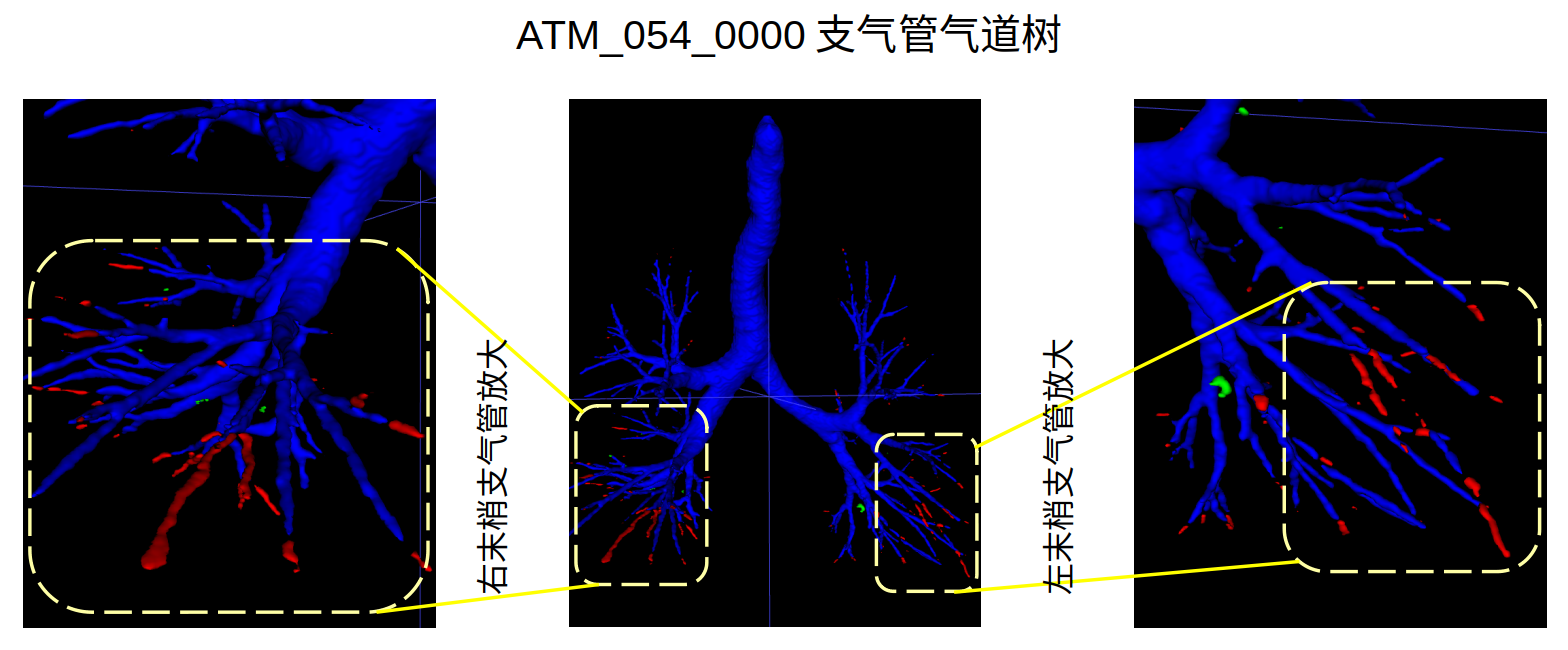
\includegraphics[width=\textwidth]{zoom_in_distal_bronchus}
    \bicaption[末梢支气管出现假阴性分割效果]
        {末梢支气管出现假阴性分割效果}
        {The distal bronchus segmentation showed false-negative voxels}
    \label{fig:distal_bronchus}
\end{figure}
末梢支气管的管径通常都比较小,做标注工作的临床医生在标注这些末梢支气管尽很大的努力,可能只能看到一到两个像素。ATM\_054\_0000切片上
的像素间距是0.83mm,切片间距是0.5mm,由此可见末端支气管的管径在人体肺部实际不到1mm。 对于医生来说,精细标注确实是一个比较大
的挑战,大量CT图片的精细标注是一项繁重耗时且枯燥乏味的工作。但对于支气管镜导航手术来说,越是进入末梢支气管越能接近肺癌结节
部位,越好做到微创甚至无创取样活检。这就要求我们做支气管气道树分割越精细越好,较高要求是能分割到段支气管、小叶支气管。当然最高要求是做到
能分割细支气管,细支气管是最末端的毛细支气管,直接连到肺泡。

对于卷积网络提取精细特征的要求,Sergey Zagoruyko等人\cite{Zagoruyko2016PayingMA}提出卷积网络注意力转移Attention Transfer
的方法,注意力转移将知识从教师网络转移到学生网络,可以改善CNN的分割性能。 Geoffrey Hinton和Jeff Dean等人\cite{Hinton2015DistillingTK}
提出知识蒸馏的概念,指出注意力图是一种有价值的知识。受此启发,知识可迁移,注意力帮助聚焦,我们提出注意力蒸馏的方法。在学习支气管
气道树的特征时,加强对末梢支气管这些细小对象的关注,可帮助提高3D-UNet网络的分割性能。

\section{注意力蒸馏方法}

注意力是一组空间地图,本质是试图使网络在做出输出决策时最关注的输入空间区域\cite{Zagoruyko2016PayingMA}。有两种注意力图
的形式,一种是基于激活的注意力图Activation-based attention map, 另一种是基于梯度的注意力图Gradient-based 
attention map. 这种注意力图可在网络的各个层定义,以便它们能够捕获低级、中级和高级别的表示信息。注意力图可指导我们看哪里,
把目光聚焦在感兴趣的地方。 

在卷积网络的第$n$层,定义注意力图$\mathit{AttMap}_{n}$作用在该层特征$\mathit{Feat}_{n}$的函数关系:
\begin{equation}\label{eq:attention_map}
    \mathcal{F}: \mathit{Feat}_{n}^{C \times D \times H \times W} \longrightarrow \mathit{AttMap}_{n}^{1 \times D \times H \times W}
\end{equation}
这里上标$D \times H \times W$表示维数,因为3D-UNet是以三维长方体子块体数据为输入的,就像UNet以二维的图像数据为输入的。
二维图像数据的维度是$Height \times Width$,三维长方体子块体数据的维度是$Depth \times Height \times Width$。而$C$
表示通道维数,也就是在第$n$层卷积有$C$个$D \times H \times W$个长方体子块。

如何计算\ref{eq:attention_map}式的函数关系? Sergey Zagoruyko等人在论文\textit{Paying more attention to Attention: 
Improving the performance of convolutional neural networks via Attention Transfer}中提出了三种计算方式
\cite{Zagoruyko2016PayingMA}:
\begin{enumerate}
    \item 沿着通道维数,计算绝对值之和  
    \begin{equation}
        \mathcal{F}_{sum}(\mathit{Feat}_{n}) = \sum_{c=1}^{C}{\Bigm| \mathit{Feat}_{n}\Bigm|}
    \end{equation}
    
    \item 沿着通道维数,计算绝对值的$p$次幂之和
    \begin{equation}
        \mathcal{F}_{sum}^{p}(\mathit{Feat}_{n}) = \sum_{c=1}^{C}{\Bigm| \mathit{Feat}_{n} \Bigm|}^{p}
    \end{equation}
    
    \item 沿着通道维数,计算绝对值的$p$次幂的最大值
    \begin{equation}
        \mathcal{F}_{max}^{p}(\mathit{Feat}_{n}) = \max_{c=1}^{C}{\Bigm| \mathit{Feat}_{n} \Bigm|}^{p}
    \end{equation}
\end{enumerate}
在这里我们选择第2种计算方式,沿着通道维数,计算绝对值的$p$次幂之和。因为这种计算方式保留了该层特征的所有隐含的显著激活信息,
但不会忽略非最大的元素,也不会削弱判别性的元素。$p$次幂建议取$p = 2$, 它增强了大多数敏感任务区域。$\mathcal{F}_{sum}^{p}({Feat}_{n})$
的计算相比于$\mathcal{F}_{sum}(\mathit{Feat}_{n})$,它把更多的权重放置于最具判别性的部位。$p$越大,越能聚焦于这些判别性部位。

借助于PyTorch的张量表示方法,我们将注意力图函数改写成如下形式:
\begin{equation}
    \mathit{AttMap}_{n} = \mathcal{F}_{sum}^{p}(\mathit{Feat}_{n}) = \sum_{c=1}^{C}{\Bigm|{\mathit{Feat}}[c, :, :, :]\Bigm|}^{p}
\end{equation}
其中$\mathit{Feat}[c, :, :, :]$表示通道维$c$、 深度维$D$全部索引、 高度维$H$全部索引、宽度维$W$全部索引, 后面的$[:, :, :]$就构成了一个$D \times H \times W$的
长方体子块。

这种计算注意力图的方式其意义就是将$C$个$D \times H \times W$长方体子块的特征信息蒸馏浓缩在一个$D \times H \times W$长方体
子块特征里。如图\ref{fig:attention_distillation}所示:
\begin{figure}[!htp]
    \centering
    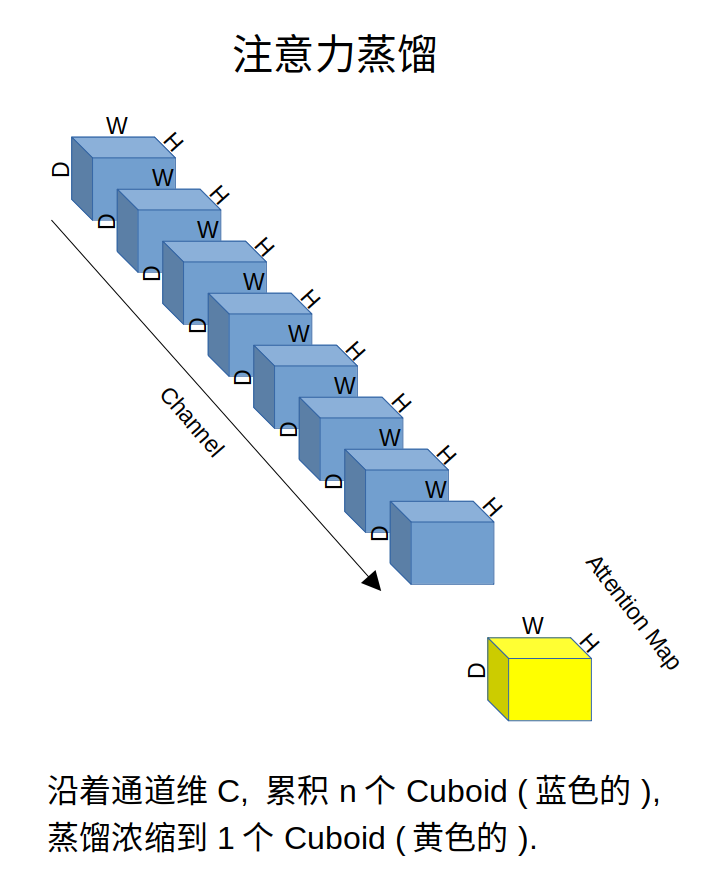
\includegraphics[width=0.6\textwidth]{Attention_Distillation}
    \bicaption[注意力蒸馏的原理]
        {注意力蒸馏的原理}
        {How the attention distillation works}
    \label{fig:attention_distillation}
\end{figure}

为了保证蒸馏得到的注意力图Cuboid与原来的特征Cuboid保持相同的$D \times H \times W$维数,我们需要对注意力图进行三线性
插值Trilinear Interpolation $\mathcal{L}(\bullet)$
\begin{equation}
    \mathit{AttMap}_{n} = \mathcal{L}\left[\mathcal{F}_{sum}^{p}\left(\mathit{Feat}_{n}\right)\right]
\end{equation}

最后,我们使用$Softmax$对其归一化,使每个体素的值被限定在$[0, 1]$之间。
\begin{equation}
    \mathit{AttMap}_{n} = \mathit{Softmax}\{ \mathcal{L}\left[\mathcal{F}_{sum}^{p}\left(\mathit{Feat}_{n}\right)\right] \}
\end{equation}

注意力图的引入给卷积网络的层与层之间相当于增加了一个额外的梯度,使相邻两层之间更接近,可以使$\mathit{AttMap}_{n}$与$\mathit{AttMap}_{n+1}$
之差最小化,即它们的累积损失最小。
\begin{equation}\label{eq:attention_distillation_loss}
    \mathit{Loss} = \min \sum_{n=1}^{N-1} \Bigm|\Bigm|\mathit{AttMap}_{n} - \mathit{AttMap}_{n+1} \Bigm|\Bigm|_{F}^{2}
\end{equation}
其中$\Bigm|\Bigm|\bullet\Bigm|\Bigm|_{F}$是指矩阵的Frobenius范数。

以上是注意力图的计算过程。引入注意力蒸馏的目的是为了增加对细颗粒度的物体的关注,在本文中就是为了增加对末梢支气管这些细小的支气管
体素的关注,从而提高分割的性能。

\section{注意力蒸馏的效果可视化}

引入注意力蒸馏方法后,我们可以来看看在卷积网络不同层之间,经过蒸馏后特征的表现如何? 通过可视化的方式来查看支气管气道树的焦点
变化情况。我们选取了测试集的ATM\_074\_0000这个病例,抽取3D-UNet结构图\ref{fig:3DUNetStructure}上采样路径的第6、第7、
第8、第9个卷积层的特征信息,将它们显示出来,如图\ref{fig:ad_effect}所示。
\begin{figure}[ht]
    \centering
    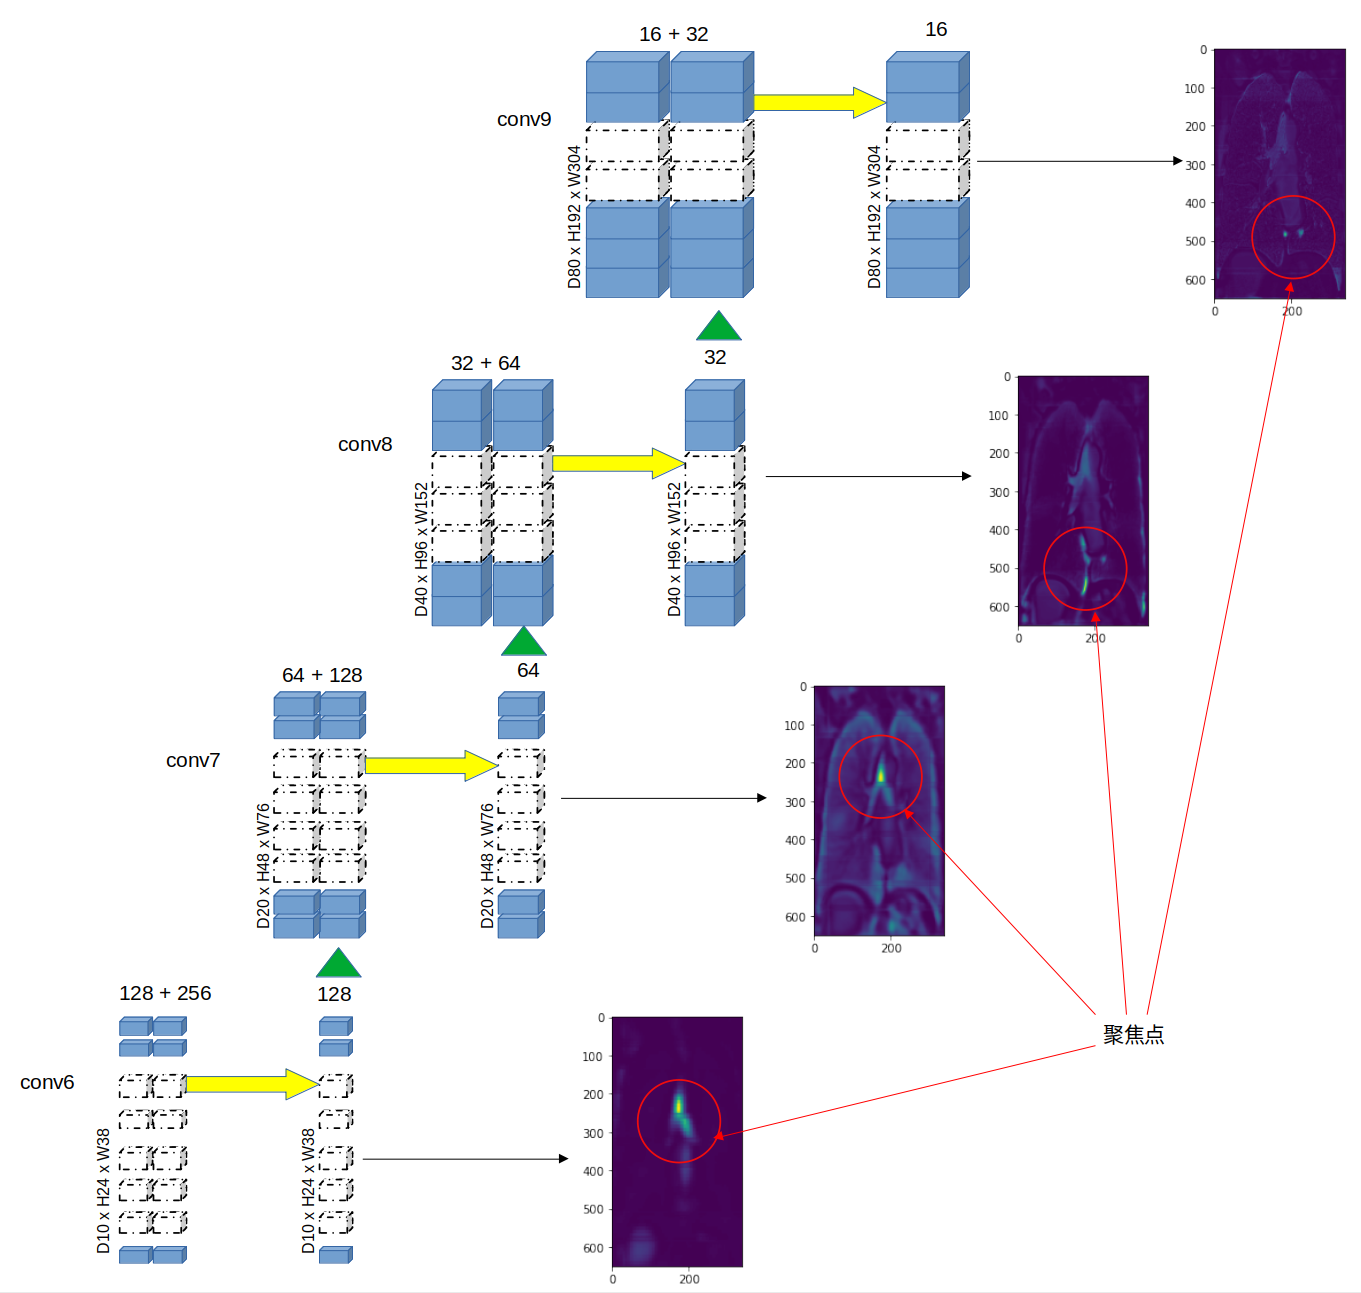
\includegraphics[width=\textwidth]{visualize_attention_distillation_effect}
    \bicaption[注意力蒸馏后的效果]
        {注意力蒸馏后的效果}
        {The visual effect of feature after attention distillation}
    \label{fig:ad_effect}
\end{figure}
从图\ref{fig:ad_effect}可以看出,高亮之处也就是聚焦点沿着conv6->conv7->conv8->conv9的方向从粗壮的气管逐渐转移至更
细小的末梢支气管,这也是注意力机制在引导我们聚焦看哪里。为了更清晰,我们将注意力蒸馏后的图片转成灰度图并放大,请见图\ref{tbl:ad_effect},
对比4个卷积层蒸馏后焦点转移情况。说明一点,为了便于读者复现此注意力蒸馏后的效果,显示如图\ref{tbl:ad_effect}的图片,请参考
附录\ref{code:ad_effect}的代码片段。
%\begin{table}[!htp]
%    \centering
%    \bicaption[注意力蒸馏后图像特征对比]
%        {注意力蒸馏后图像特征对比}
%        {The comparison of image feature after attention distillation}
%    \label{tbl:ad_effect}
%    \scalebox{0.8}{
%    \begin{tabular}{|c|c|}
%        \hline
%        第6个卷积层蒸馏后 & 第7个卷积层蒸馏后 \\
%        \hline
%        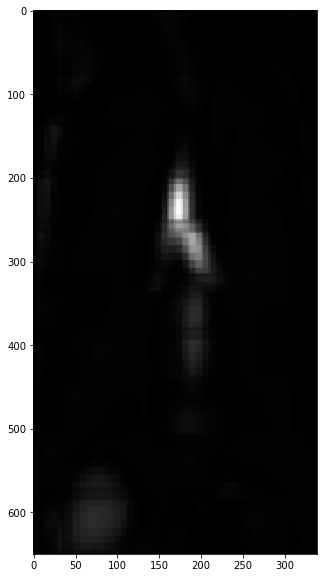
\includegraphics[width=0.5\textwidth, height=0.55\textheight]{Illustration/ad_feat6} & 
%        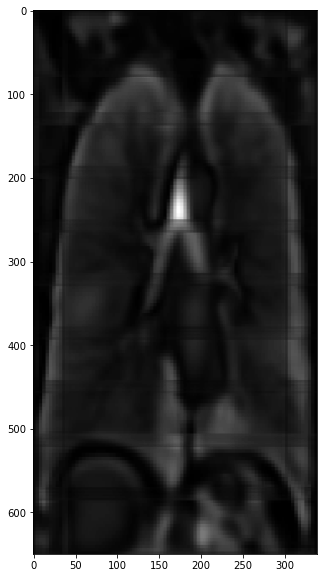
\includegraphics[width=0.5\textwidth, height=0.55\textheight]{Illustration/ad_feat7} \\
%        \hline
%        第8个卷积层蒸馏后 & 第9个卷积层蒸馏后 \\
%        \hline
%        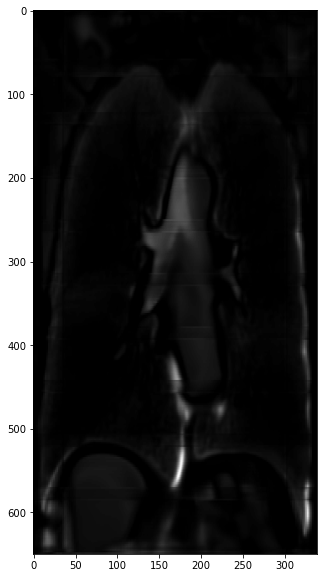
\includegraphics[width=0.5\textwidth, height=0.55\textheight]{Illustration/ad_feat8} & 
%        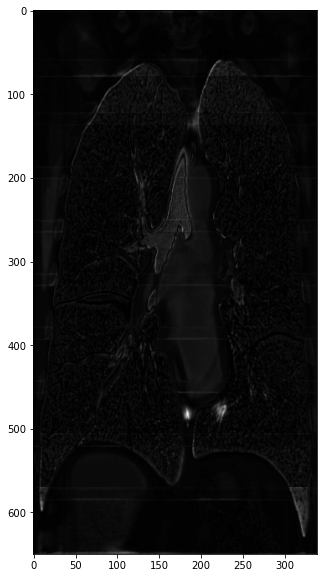
\includegraphics[width=0.5\textwidth, height=0.55\textheight]{Illustration/ad_feat9} \\
%        \hline
%    \end{tabular}}
%\end{table}

\begin{figure}[!htp]
	\centering
	\begin{subfigure}{0.45\textwidth}
		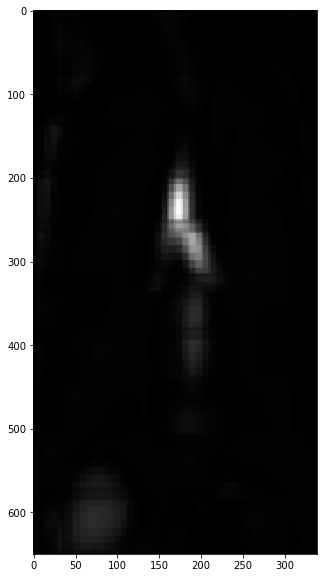
\includegraphics[width=\textwidth, height=0.42\textheight]{Illustration/ad_feat6}
		\caption{第6个卷积层蒸馏后}
	\end{subfigure}
	\hfill
	\begin{subfigure}{0.45\textwidth}
		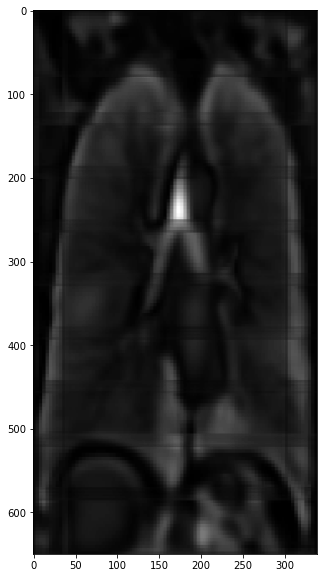
\includegraphics[width=\textwidth, height=0.42\textheight]{Illustration/ad_feat7}
		\caption{第7个卷积层蒸馏后}
	\end{subfigure}
	\\
	\begin{subfigure}{0.45\textwidth}
		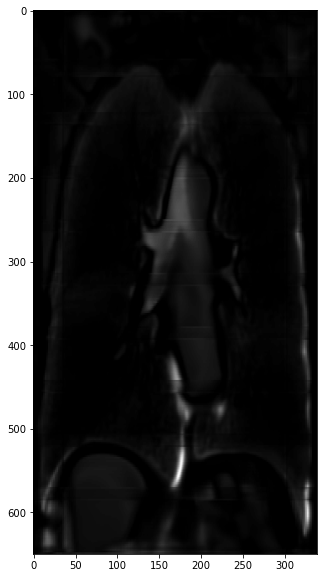
\includegraphics[width=\textwidth, height=0.42\textheight]{Illustration/ad_feat8}
		\caption{第8个卷积层蒸馏后}
	\end{subfigure}
	\hfill
	\begin{subfigure}{0.45\textwidth}
		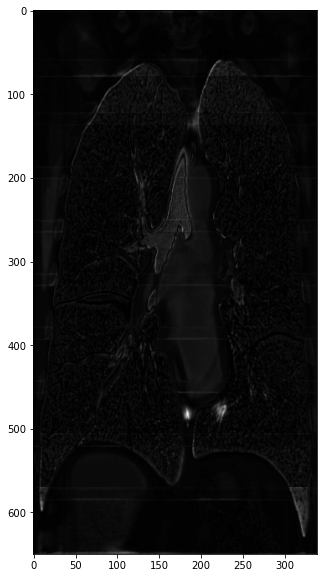
\includegraphics[width=\textwidth, height=0.42\textheight]{Illustration/ad_feat9}
		\caption{第9个卷积层蒸馏后}
	\end{subfigure}
	\bicaption[注意力蒸馏后图像特征对比]
        {注意力蒸馏后图像特征对比}
        {The comparison of image feature after attention distillation}
	\label{tbl:ad_effect}
\end{figure}

注意力蒸馏方法可使焦点转移,聚焦于看更细节的对象,帮助模型提高精细度的性能。为此,我们对前文的3D-UNet基准网络进行改进,引入
注意力蒸馏方法。

\section{引入注意力蒸馏模块对3D-UNet基准网络进行改进}
基于前文对注意力蒸馏方法的研究,我们决定对3D-UNet基准网络进行改进,引入注意力蒸馏方法,在3D-UNet上采样路径上对第6个、第7个、
第8个和第9个卷积层添加注意力蒸馏模块。经过注意力蒸馏模块后,相邻的蒸馏后图像特征之间就自然增加了一个新的梯度,我们通过
\ref{eq:attention_distillation_loss}式来计算它们之间的损失。

改进后的网络结构如图\ref{fig:3dunet_ad}所示。因插图横向宽度太长,将其横向放置,利于看清图中细小的字体。
\begin{figure}[!ht]
    \centering
    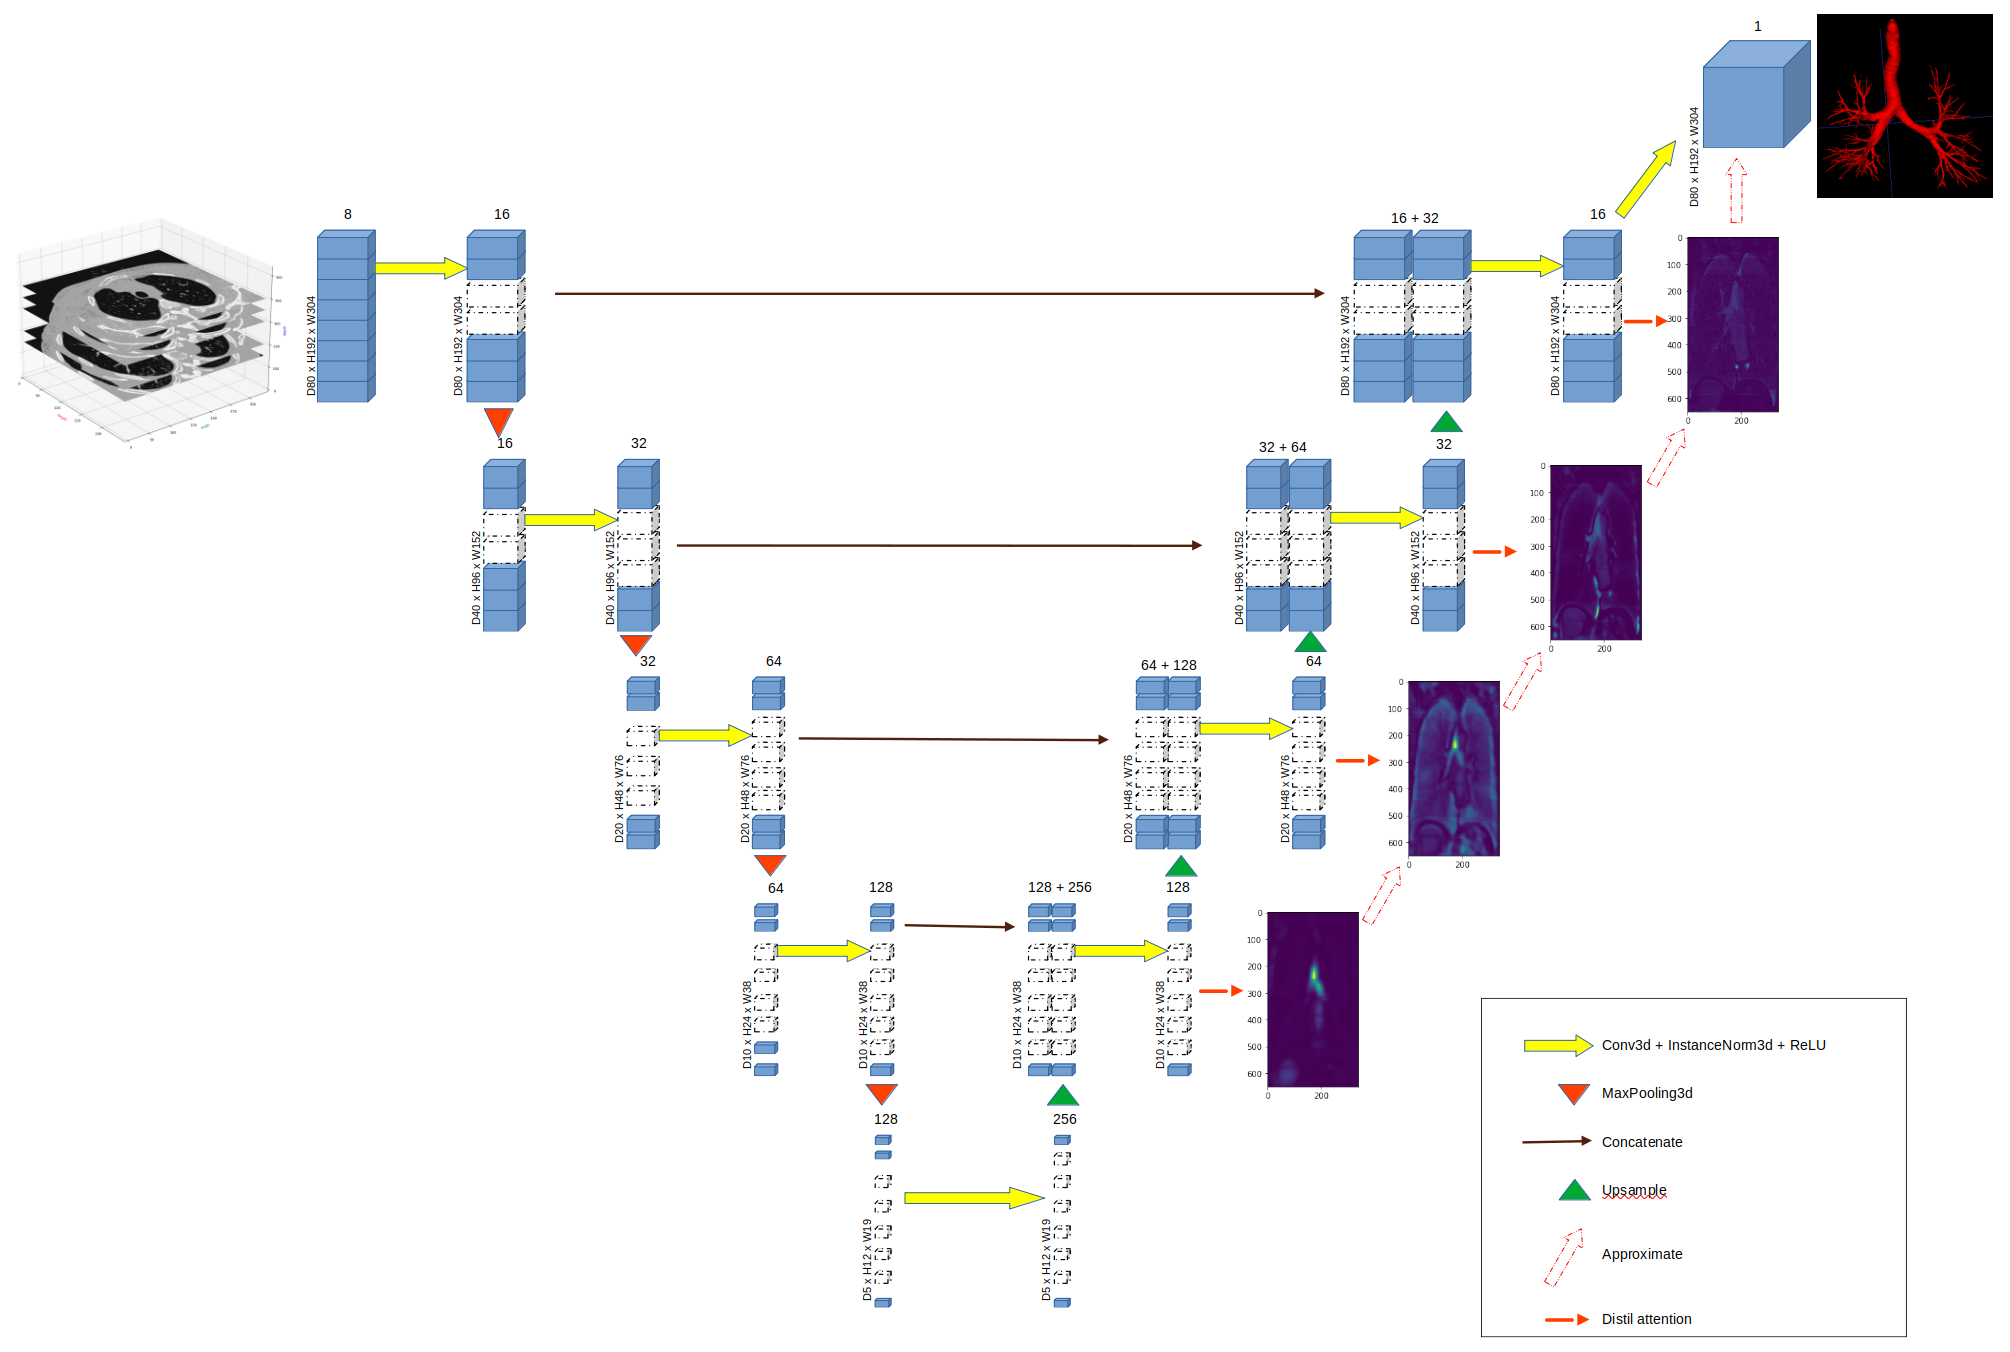
\includegraphics[width=0.83\textheight, height=\textwidth, angle=90]{Baseline_AD}
    \bicaption[3D-UNet + Attention Distillation网络结构示意图]
        {3D-UNet + Attention Distillation网络结构示意图}
        {The architecture of 3D-UNet + Attention Distillation}
    \label{fig:3dunet_ad}
\end{figure}
我们只是在上采样路径上加入了注意力蒸馏模块,而并没有在下采样路径上同样加入注意力蒸馏模块,为什么? 这是考虑到下采样路径上第$n$
个卷积层本身就比第$n-1$个卷积层的输出图像的分辨率要低,这就必然导致末梢支气管的像素密度更低。在低分辨率下,注意力蒸馏就很难聚焦
于末梢支气管,所以就难以起到正向促进作用。而在上采样路径则正好相反,第$n$个卷积层比第$n-1$个卷积层的图像分辨率提高一倍,末梢
支气管的像素密度高,那么注意力蒸馏就可以比较容易地聚焦于这些末梢支气管。

对于注意力蒸馏模块引入后额外增加的梯度,其带来的损失函数的计算,实现算法~\ref{algo:ad_loss},需要累积各个卷积层的注意力
\begin{algorithm}[htb]
    \SetKwData{pred}{pred}
    \SetKwData{gt}{groundtruth}
    \SetKwFunction{len}{length}
    \SetKwFunction{interpolate}{torch.nn.functional.interpolate}
    \SetKwData{scalefactor}{scale\_factor=2}
    \SetKwData{mode}{mode='trilinear'}
    \SetKwFunction{size}{size}
    \SetKwData{flattenpred}{flatten\_pred}
    \SetKwData{flattengt}{flatten\_gt}
    \SetKwFunction{view}{view}
    \SetKwData{predsoftmax}{pred\_softmax}
    \SetKwData{gtsoftmax}{groundtruth\_softmax}
    \SetKwFunction{softmax}{torch.nn.functional.softmax}
    \SetKwData{dim}{dim=1}
    \SetKwData{loss}{loss}
    \SetKwFunction{mseloss}{torch.nn.functional.mse\_loss}
    
    \caption{注意力蒸馏的梯度损失}
    \label{algo:ad_loss}
    \small
    \SetAlgoLined
    \KwData{$AttMap[4]$, $\gamma[3]$}
    \KwResult{$Total\_Loss$}
    
    $Total\_Loss \leftarrow 0$
    \BlankLine
    $\gamma[3] \leftarrow [0.1, 0.1, 0.1]$
    \BlankLine
    
    \For{$i \leftarrow 0$ \KwTo \len{$AttMap$}-1 }{
        \pred $\leftarrow$ $AttMap[i]$
        \BlankLine
        \gt $\leftarrow$ $AttMap[i+1]$
        \BlankLine
        \pred $\leftarrow$ \interpolate{\pred, \mode, \scalefactor}
        \BlankLine
        
        $N$ = \pred.\size{0}
        \BlankLine
        \flattenpred $\leftarrow$ \pred.\view{$N$, -1}
        \BlankLine
        \flattengt $\leftarrow$ \gt.\view{$N$, -1}
        \BlankLine
        \predsoftmax $\leftarrow$ \softmax{\flattenpred, \dim}
        \BlankLine
        \gtsoftmax $\leftarrow$ \softmax{\flattengt, \dim}
        \BlankLine
        
        \loss $\leftarrow$ \mseloss{\predsoftmax, \gtsoftmax}
        \BlankLine
        
        $Total\_Loss \leftarrow$ $Total\_Loss$ + $\gamma[i]$ * \loss
    }
\end{algorithm}
蒸馏的梯度损失。骰子损失Dice Loss还是按照\ref{eq:dice_loss}式进行计算,Focal Loss损失按照公式\ref{eq:focal_loss}计算,
最后需要将此计算出来的总的注意力蒸馏的梯度损失缀加到Total Loss(见公式\ref{eq:total_loss})上。需要指出的是,注意力蒸馏的梯度损失函数是可微可导的,因此在误差反向
传播时是可以更新3D-UNet网络的参数的。

\section{对比实验与实验结果分析}
我们对3D-UNet基准网络进行改进,加入了注意力蒸馏模块后,现在我们进行一次实验,与前文的3D-UNet基准网络实验进行对比。使用的
数据集与3D-UNet实验的数据集完全相同,实验条件也是一致的。本次实验的训练、验证和测试三个阶段合计总耗时约39个小时。

验证集的指标数据如表\ref{tbl:3dunet_ad_metrics_valset}所示。
\begin{table}[htb]
    \centering
    \bicaption[3D-UNet + AD网络结构的验证集指标数据一览表]
        {3D-UNet + AD网络结构的验证集指标数据一览表\\表中每一项指标栏用双下划线加粗黑体标示出表现最优秀的, 
        用波浪线标示出表现最差的.}
        {The metrics overview of validate set under 3D-UNet + AD network structure}
    \label{tbl:3dunet_ad_metrics_valset}
    \begin{tabular}{cccccccc}
        \toprule
        病例名称 & FPR & FNR & Sensitivity & Precison & DSC & BD & TLD \\
        \midrule
        ATM\_029\_0000 & 0.022 & 9.266  & 90.734 & 91.012 & \uwave{90.87} & 76.92  & 85.85  \\
        ATM\_054\_0000 & 0.037 & 3.499  & 96.501 & 92.319 & 94.36 & 76.16  & \uwave{83.93}  \\
        ATM\_055\_0000 & 0.039 & 3.453  & 96.547 & 89.855 & 93.08 & 81.17  & 89.09  \\
        ATM\_057\_0000 & 0.039 & 4.683  & 95.317 & 90.426 & 92.81 & 78.35  & 87.98  \\
        ATM\_091\_0000 & \uwave{0.041} & 3.57   & 96.43  & \uwave{89.583} & 92.88 & 85.46  & 91.99  \\
        % ATM\_174\_0000 & 0.031 & 21.972 & 78.028 & 91.218 & 84.11 & 38.1   & 49.49  \\
        ATM\_215\_0000 & \uuline{\bf 0.021} & \uwave{10.595} & \uwave{89.405} & \uuline{\bf 92.453} & 90.9  & \uwave{72.25}  & 84.32  \\
        % ATM\_505\_0000 & 0.061 & 44.617 & 55.383 & 85.209 & 67.13 & 26.51  & 42.18  \\
        ATM\_688\_0000 & 0.028 & \uuline{\bf 2.109}  & \uuline{\bf 97.891} & 92.182 & \uuline{\bf 94.95} & \uuline{\bf 93.94}  & \uuline{\bf 96.31}  \\
        \midrule
        平均值 & 0.032 & 5.311 & 94.689 & 91.119 & 92.836 & 80.607 & 88.496 \\
        \bottomrule
    \end{tabular}
\end{table}
另外算出这些指标的平均值,以便与3D-UNet基准网络实验的验证集的指标的平均值进行比较。

测试集的指标数据如表\ref{tbl:3dunet_ad_metrics_testset}所示。从平均值来看,FPR、Sensitivity、DSC和TLD四项指标表现得都比较优秀。
\begin{table}[!htb]
    \centering
    \bicaption[3D-UNet + AD网络结构的测试集指标数据一览表]
        {3D-UNet + AD网络结构的测试集指标数据一览表\\表中每一项指标栏用双下划线加粗黑体标示出表现最优秀的, 
        用波浪线标示出表现最差的.}
        {The metrics overview of testset under 3D-UNet + AD network structure}
    \label{tbl:3dunet_ad_metrics_testset}
    \begin{tabular}{cccccccc}
        \toprule
        病例名称 & FPR & FNR & Sensitivity & Precison & DSC & BD & TLD \\
        \midrule
        ATM\_001\_0000 & \uuline{\bf 0.007} & 7.258  & 92.742 & \uuline{\bf 97.779} & 95.19  & 71.05   & 85.1   \\
        ATM\_024\_0000 & 0.036 & 6.387  & 93.613 & 89.696 & 91.61  & 87.54   & 93.5   \\
        ATM\_034\_0000 & 0.021 & 4.039  & 95.961 & 96.455 & \uuline{\bf 96.21}  & 93.06   & 94.67  \\
        ATM\_041\_0000 & 0.055 & 4.486  & 95.514 & 85.247 & 90.09  & 83.42   & 90.69  \\
        ATM\_060\_0000 & 0.027 & 2.682  & 97.318 & 92.505 & 94.85  & 90.17   & 94.34  \\
        ATM\_061\_0000 & 0.034 & 3.152  & 96.848 & 90.471 & 93.55  & 85.05   & 90.35  \\
        ATM\_074\_0000 & 0.06  & 2.934  & 97.066 & 85.671 & 91.01  & 91.64   & 94.44  \\
        ATM\_075\_0000 & 0.027 & 3.944  & 96.056 & 92.649 & 94.32  & 88.68   & 92.16  \\
        ATM\_080\_0000 & 0.031 & 3.662  & 96.338 & 92.216 & 94.23  & 78.55   & 88.01  \\
        ATM\_150\_0000 & \uwave{0.085} & 3.853  & 96.147 & \uwave{79.511} & \uwave{87.04}  & 74.78   & 88.6   \\
        ATM\_158\_0000 & 0.047 & 3.003  & 96.997 & 86.234 & 91.3   & 87.87   & 92.67  \\
        ATM\_163\_0000 & 0.039 & 3.726  & 96.274 & 91.247 & 93.69  & 88.06   & 94.41  \\
        ATM\_197\_0000 & 0.032 & \uwave{10.332} & \uwave{89.668} & 90.723 & 90.19  & \uwave{64.03}   & \uwave{81.64}  \\
        ATM\_245\_0000 & 0.036 & \uuline{\bf 0.568}  & \uuline{\bf 99.432} & 84.172 & 91.17  & \uuline{\bf 100}     & \uuline{\bf 100}    \\
        ATM\_246\_0000 & 0.041 & 0.629  & 99.371 & 82.469 & 90.13  & \uuline{\bf 100}     & \uuline{\bf 100}    \\
        ATM\_260\_0000 & 0.019 & 1.144  & 98.856 & 93.23  & 95.96  & 98.9    & 98.71  \\
        ATM\_266\_0000 & 0.025 & 2.077  & 97.923 & 91.103 & 94.39  & \uuline{\bf 100}     & 99.24  \\
        ATM\_271\_0000 & 0.055 & 1.238  & 98.762 & 85.151 & 91.45  & 98.4    & 98.34  \\
        ATM\_638\_0000 & 0.016 & 3.52   & 96.48  & 94.514 & 95.49  & 90.48   & 95.91  \\
        \midrule
        平均值 & 0.036 & 3.612 & 96.388 & 89.529 & 92.73 & 87.983 & 93.304  \\
        \bottomrule
    \end{tabular}
\end{table}

我们还可从平均值来比较3D-UNet跟3D-UNet + AD的指标性能,见表\ref{tbl:metrics_comparison}。
\begin{table}[!hbt]
    \centering
    \bicaption[3D-UNet与3D-UNet + AD的性能指标对比]
        {3D-UNet与3D-UNet + AD的性能指标对比}
        {The metrics comparison between 3D-UNet and 3D-UNet + AD}
    \label{tbl:metrics_comparison}
    \begin{tabular}{lccccccc}
        \toprule
                & FPR & FNR & Sensitivity & Precison & DSC & BD & TLD \\
        \midrule
        \multicolumn{8}{c}{验证集} \\
        3D-UNet & {\bf 0.029} & 13.362 & 86.638 & {\bf 91.770} & 88.319 & 68.53 & 78.477 \\
        3D-UNet + AD & 0.032 & {\bf 5.311} & {\bf 94.689} & 91.119 & {\bf 92.836} & {\bf 80.607} & {\bf 88.496} \\
        \midrule
        \multicolumn{8}{c}{测试集} \\
        3D-UNet & {\bf 0.033} & {\bf 3.715} & 96.285 & {\bf 90.343} & {\bf 93.122} & 85.293 & 92.036 \\
        3D-UNet + AD & 0.036 & 3.612 & {\bf 96.388} & 89.529 & 92.73 & {\bf 87.983} & {\bf 93.304}  \\
        \bottomrule
    \end{tabular}
\end{table}
通过对比,我们看到在BD, TLD和FNR三项指标上有一些提升,在其他项指标上则基本持平。

还有一个重要的实验结果就是支气管气道树分割效果可视化,我们分别从测试集和验证中挑选一些比较有代表性的病例来展示它们的分割效果,如表
\ref{tbl:3dunetad_airway_tree}所示。
\begin{table}[!htp]
    \bicaption[3D-UNet + AD网络结构支气管气道树分割可视化3D模型]
        {3D-UNet + AD网络结构支气管气道树分割可视化3D模型\\9个样本分别从测试集和验证集挑选的}
        {Visualize the airway tree 3D models under the 3D-UNet + AD network\\The 9 samples are selected from test set and validate set.}
    \label{tbl:3dunetad_airway_tree}
    \centering
    \begin{tabular}{|c|c|c|}
        \hline
        ATM\_060\_0000 & ATM\_074\_0000 & ATM\_245\_0000 \\
        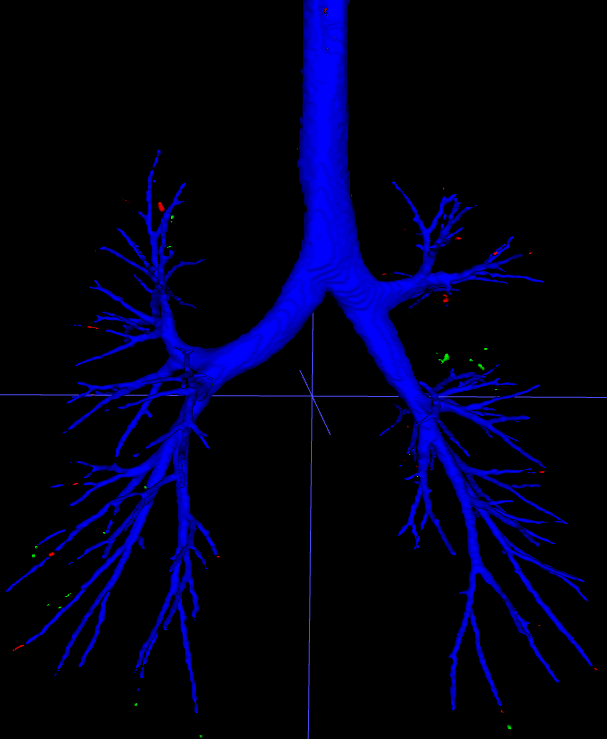
\includegraphics[width=0.3\textwidth]{results/baseline_ds_ad/test040/ATM_060_0000_airway_tree_with_3colors_at_test_epoch40} &
        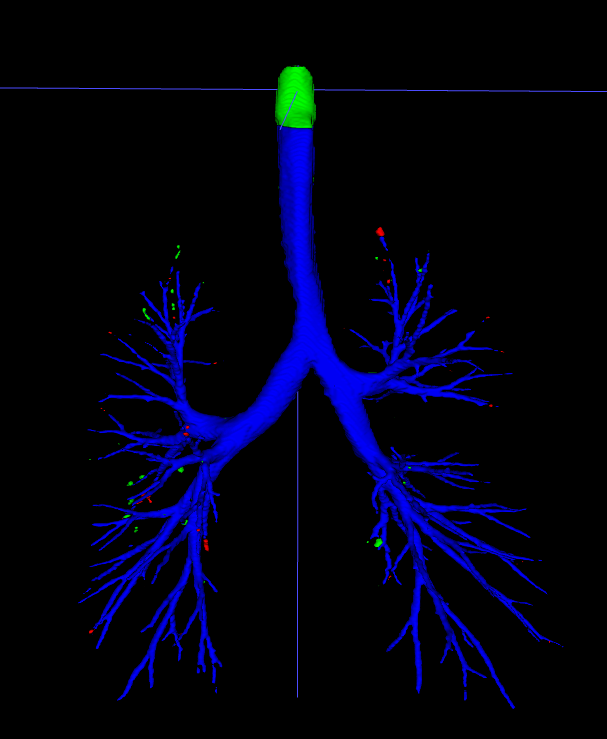
\includegraphics[width=0.3\textwidth]{results/baseline_ds_ad/test040/ATM_074_0000_airway_tree_with_3colors_at_test_epoch40} &
        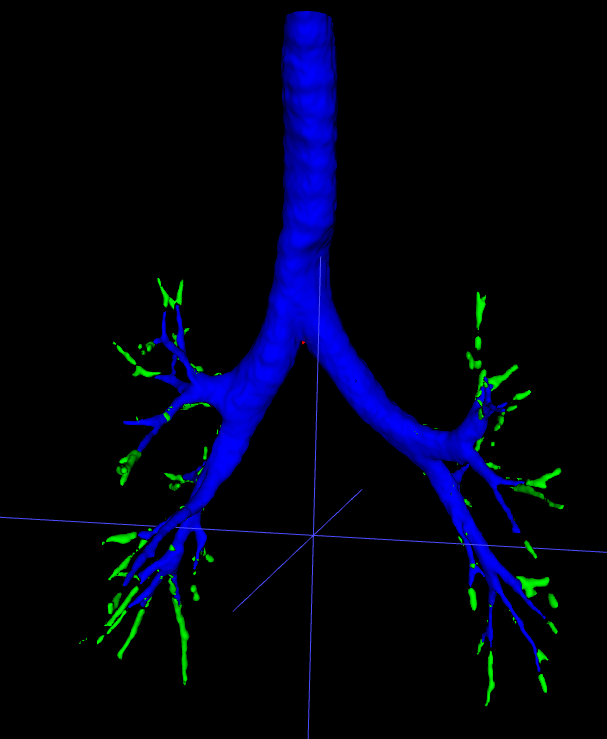
\includegraphics[width=0.3\textwidth]{results/baseline_ds_ad/test040/ATM_245_0000_airway_tree_with_3colors_at_test_epoch40} \\
        \hline
        ATM\_246\_0000 & ATM\_260\_0000 & ATM\_266\_0000 \\
        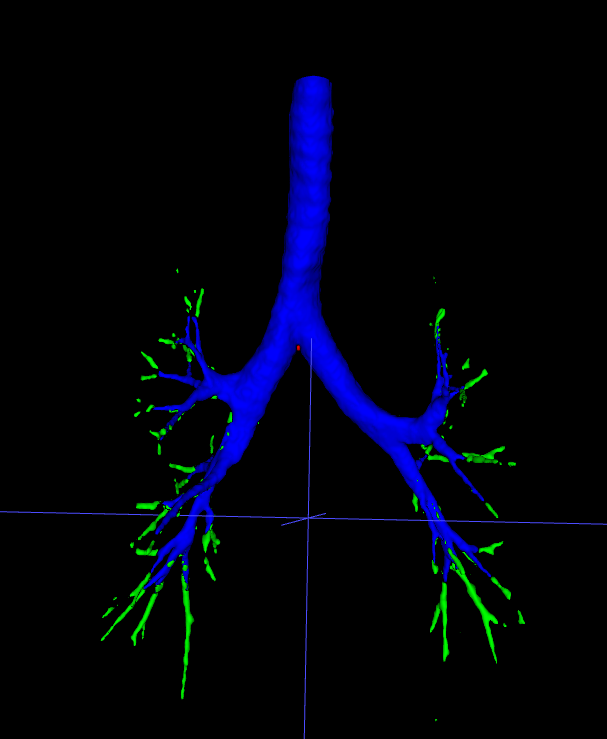
\includegraphics[width=0.3\textwidth]{results/baseline_ds_ad/test040/ATM_246_0000_airway_tree_with_3colors_at_test_epoch40} &
        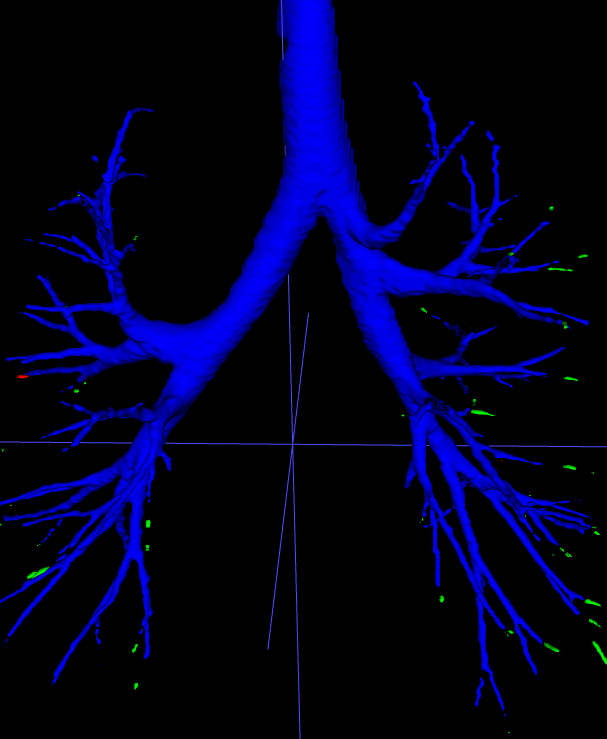
\includegraphics[width=0.3\textwidth]{results/baseline_ds_ad/test040/ATM_260_0000_airway_tree_with_3colors_at_test_epoch40} &
        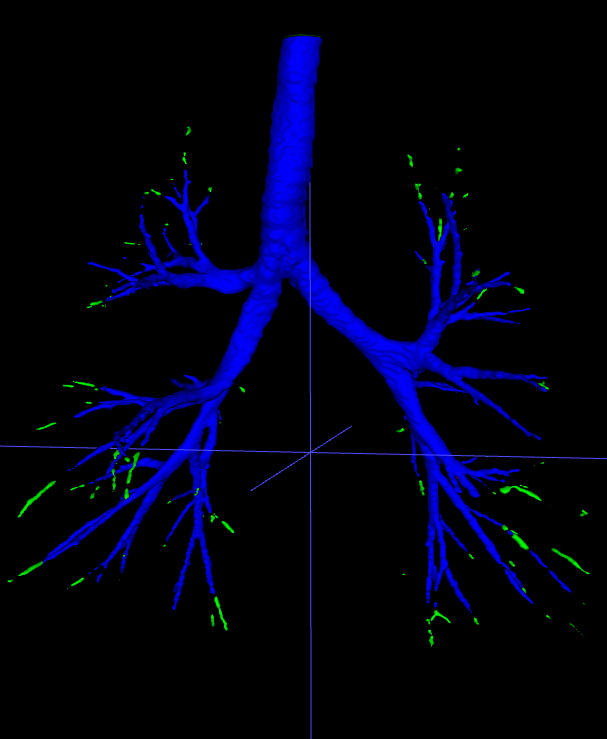
\includegraphics[width=0.3\textwidth]{results/baseline_ds_ad/test040/ATM_266_0000_airway_tree_with_3colors_at_test_epoch40} \\
        \hline
        ATM\_271\_0000 & ATM\_638\_0000 & ATM\_688\_0000 \\
        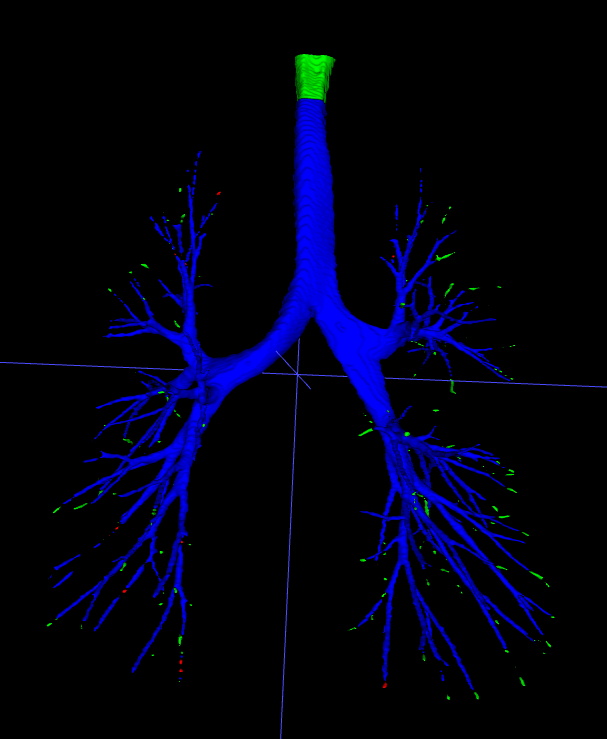
\includegraphics[width=0.3\textwidth]{results/baseline_ds_ad/test040/ATM_271_0000_airway_tree_with_3colors_at_test_epoch40} &
        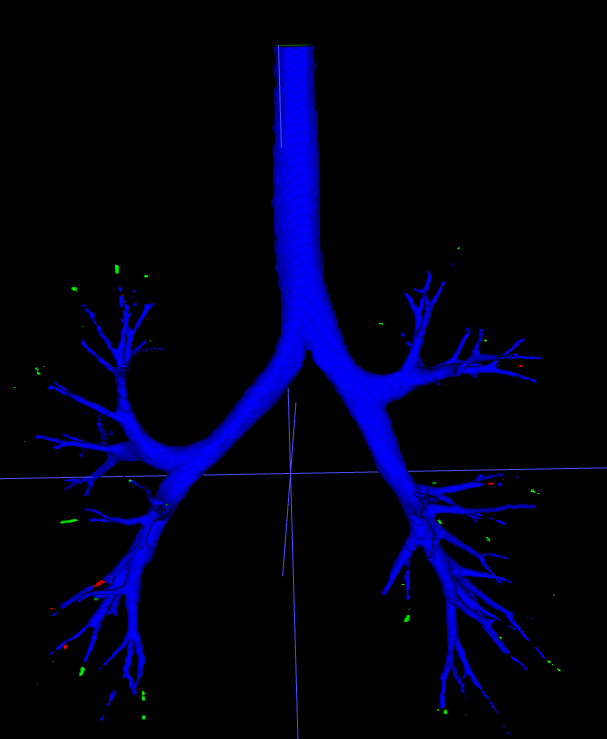
\includegraphics[width=0.3\textwidth]{results/baseline_ds_ad/test040/ATM_638_0000_airway_tree_with_3colors_at_test_epoch40} &
        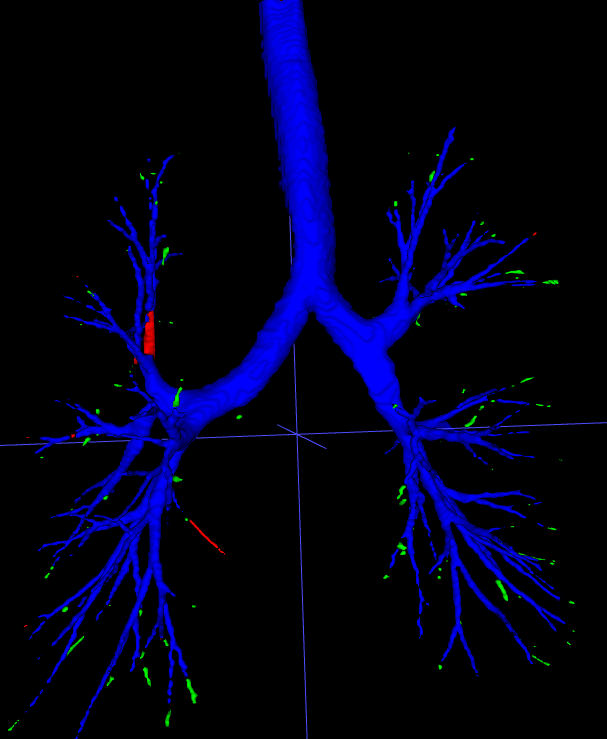
\includegraphics[width=0.3\textwidth]{results/baseline_ds_ad/val040/ATM_688_0000_airway_tree_with_3colors_at_val_epoch40} \\
        \hline
    \end{tabular}
\end{table}
从表\ref{tbl:3dunetad_airway_tree}的支气管气道树三维模型来看,大部分的假阴性(红色体素)已经被正确分割出来,9个病例中的假阴性红色体素很少出现了。
相比于表\ref{tbl:visualize_airway_3d_model}里大量出现的红色假阴性体素明显减少了很多(ATM\_174\_0000和ATM\_505\_0000两个严重肺部疾病的病例除外),证明
注意力蒸馏的方法抑制住了假阴性率,提高了分割模型的一些性能。

ATM\_688\_0000这个病例稍微有点例外,但仔细研究是在上叶支气管处出现的红色假阴性体素,上叶支气管的管径是有点粗的,分割模型应该不会在此处发生漏检,
最有可能的是医生只是标记了管内壁,没有标记管外壁。分割模型识别到管外壁,在三维支气管气道树上表现为管外壁的红色体素覆盖了馆内壁的蓝色体素。
在ITK-SNAP里放大查看,如图\ref{fig:annotation_overlap},
\begin{figure}[h]
    \centering
    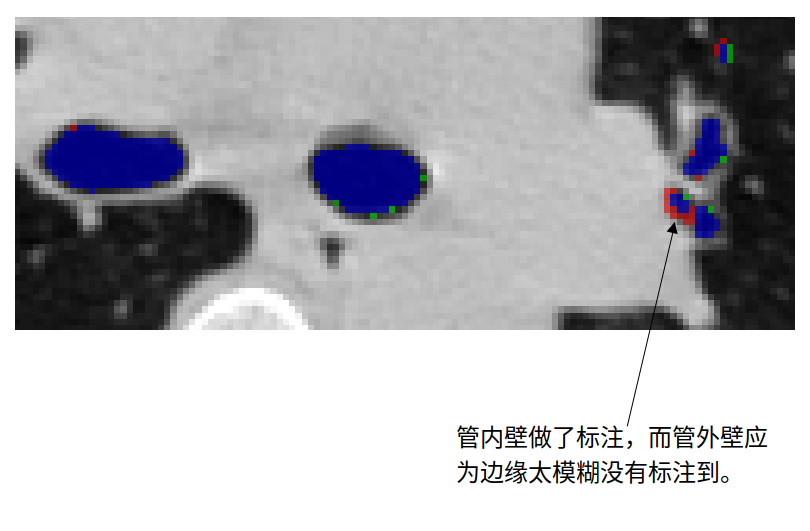
\includegraphics[width=0.5\textwidth]{results/baseline_ds_ad/管内外壁标注覆盖问题}
    \bicaption[支气管内外壁标注差异而导致覆盖问题]{支气管内外壁标注差异而导致覆盖问题}
    	{The red FN voxels outside the bronchial wall overlapped the blue TP voxels inside the bronchial wall}
    \label{fig:annotation_overlap}
\end{figure}
证实了支气管管内壁的体素被标注了,而支气管管外壁因为边缘太模糊没有标注,这就出现了管外壁的红色假阴性体素覆盖了
管内壁蓝色真阳性体素。

特别需要指出的是,ATM\_074\_0000和ATM\_271\_0000两个病例在气管最上端有非常明显的绿色假阳性体素,其实这并不是分割模型判断错误了。通过查看原始CT图像
\ref{fig:two_special_cases},确认这段绿色假阳性体素确实是咽喉处的气管。
%\begin{table}[!htp]
%    \bicaption[ATM\_074\_0000和ATM\_271\_0000两个特殊病例的分割结果分析]
%        {ATM\_074\_0000和ATM\_271\_0000两个特殊病例的分割结果分析}
%        {The segmentation results analysis for 2 special cases: ATM\_074\_0000 and ATM\_271\_0000}
%    \label{tbl:two_special_cases}
%    \centering
%    \begin{tabular}{|c|c|}
%        \hline
%        ATM\_074\_0000 & ATM\_271\_0000 \\
%        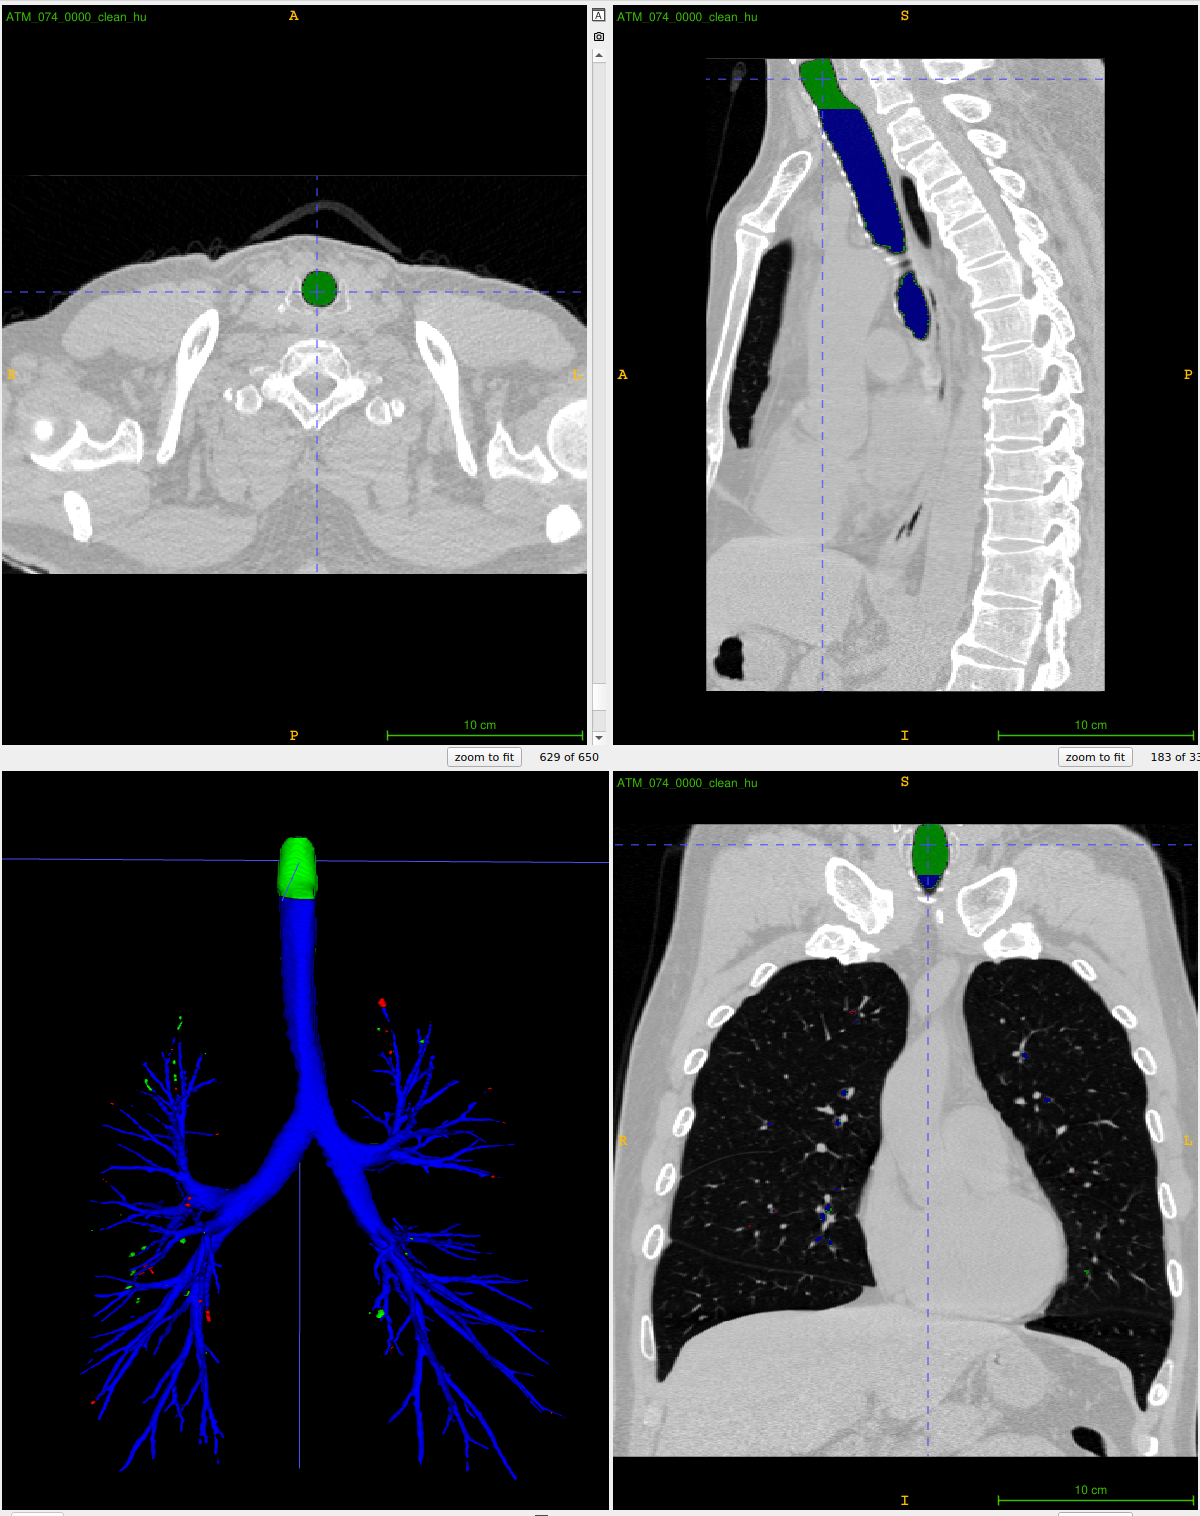
\includegraphics[width=0.45\textwidth]{results/baseline_ds_ad/test040/ATM_074_0000} &
%        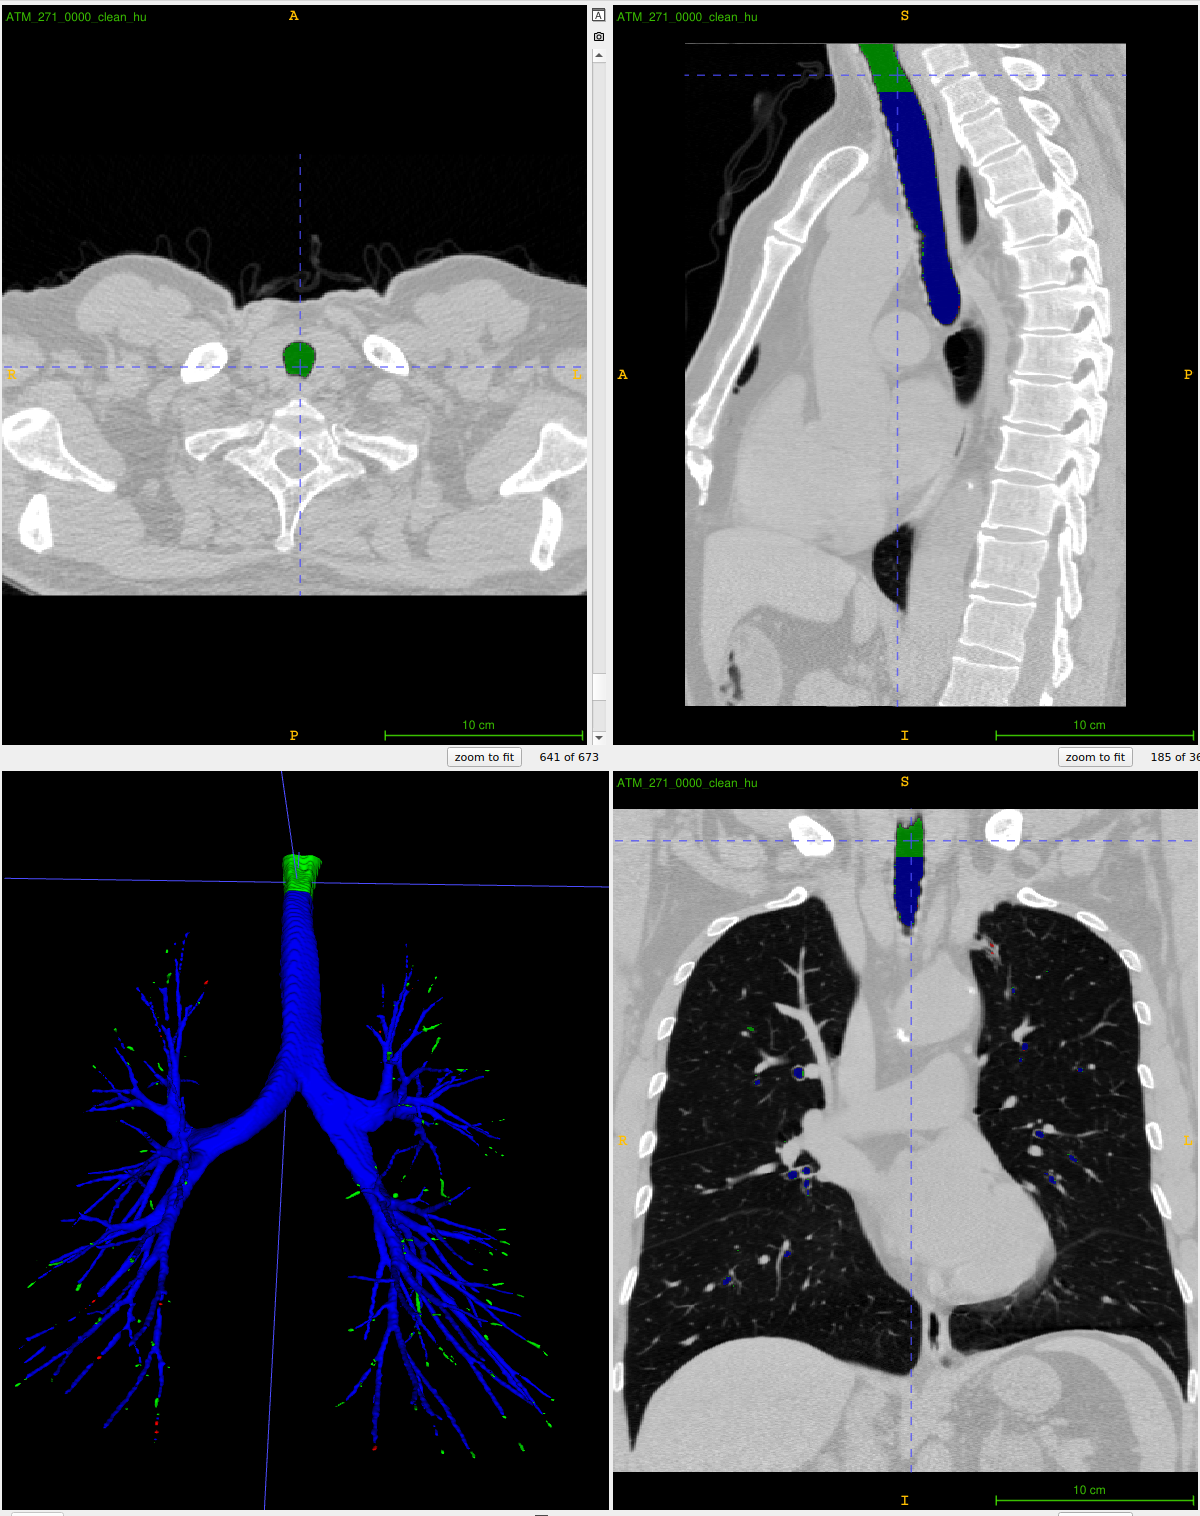
\includegraphics[width=0.45\textwidth]{results/baseline_ds_ad/test040/ATM_271_0000} \\
%        \hline
%    \end{tabular}
%\end{table}
\begin{figure}[!htp]
	\centering
	\begin{subfigure}{0.48\textwidth}
		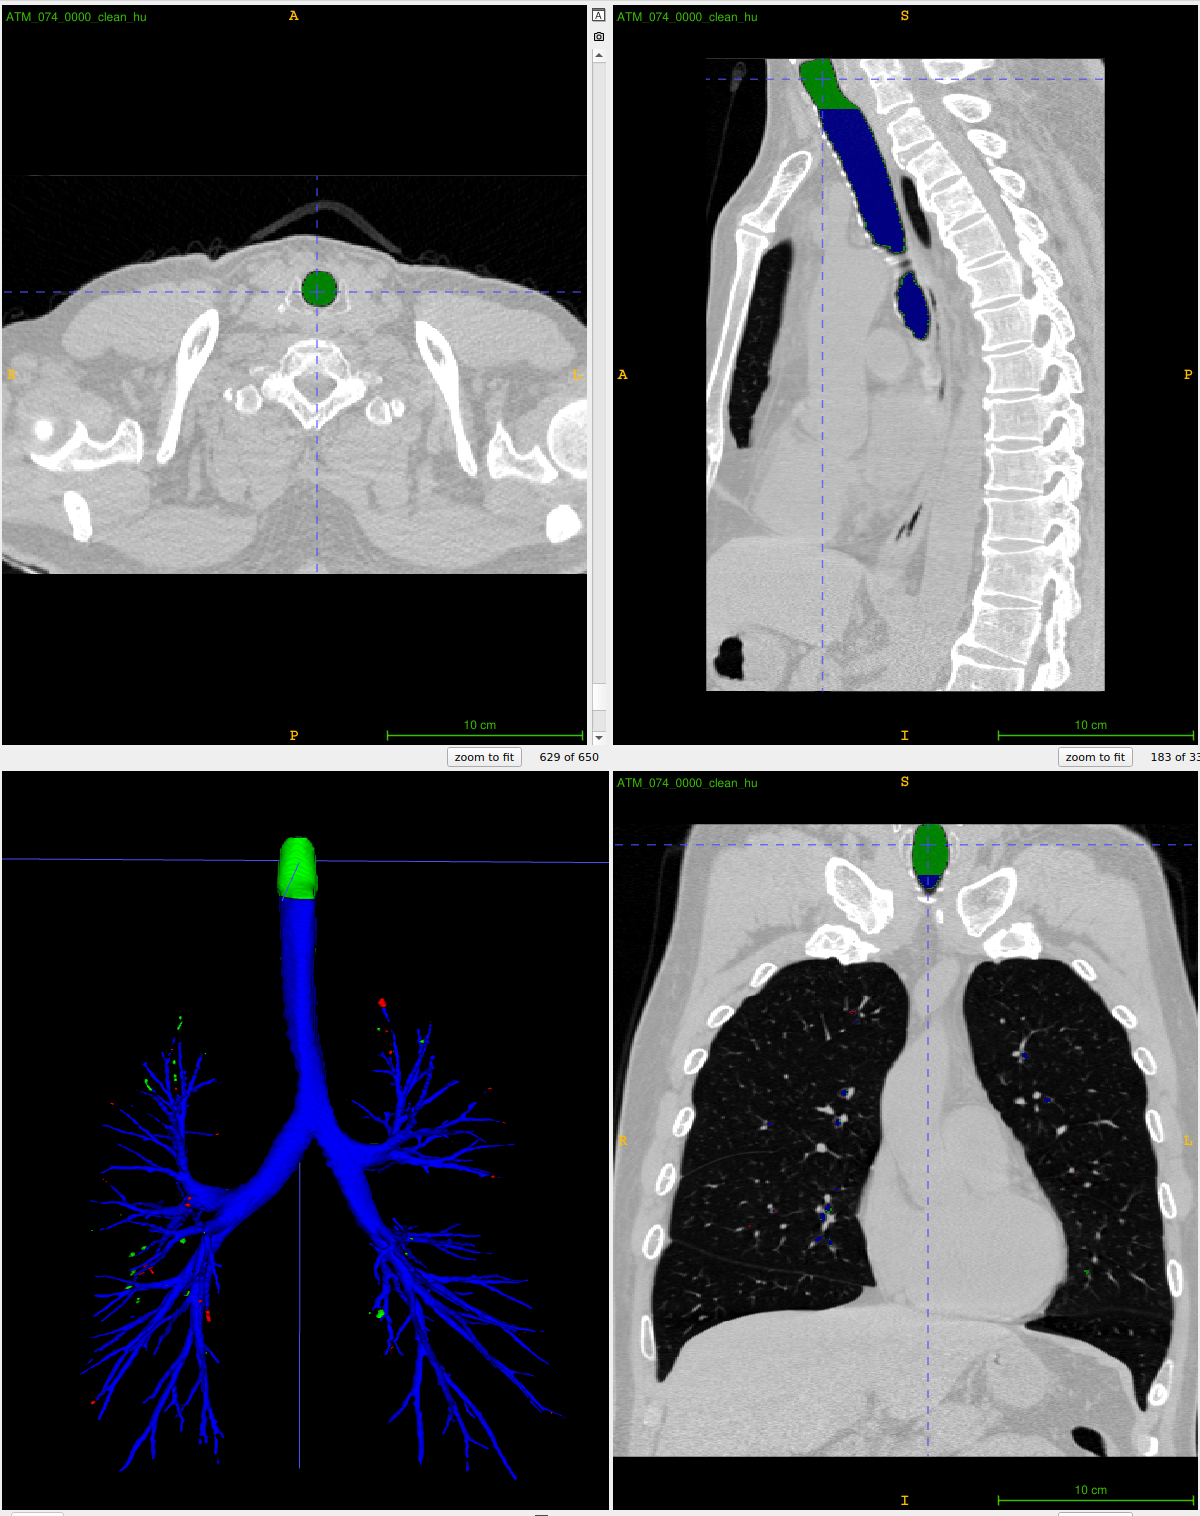
\includegraphics[width=\textwidth]{results/baseline_ds_ad/test040/ATM_074_0000}
	\end{subfigure}
	\hfill
	\begin{subfigure}{0.48\textwidth}
		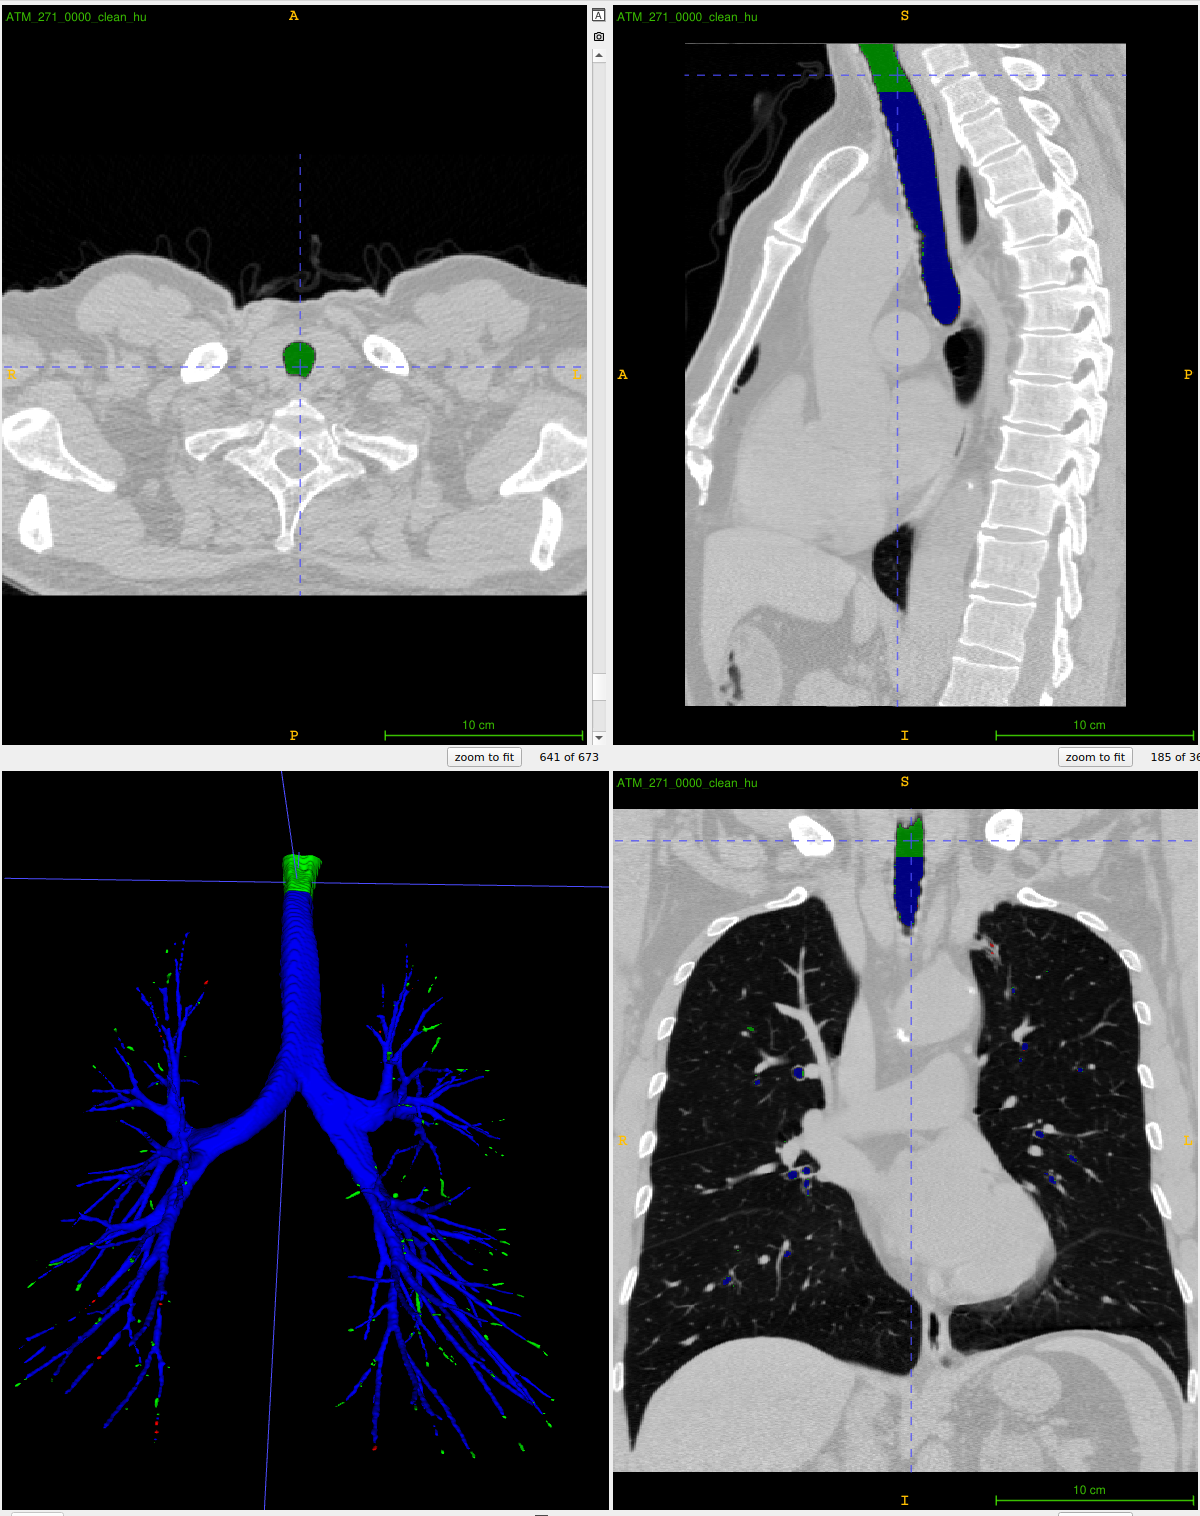
\includegraphics[width=\textwidth]{results/baseline_ds_ad/test040/ATM_271_0000}
	\end{subfigure}
	\bicaption[ATM\_074\_0000和ATM\_271\_0000两个特殊病例的分割结果分析]
        {ATM\_074\_0000和ATM\_271\_0000两个特殊病例的分割结果分析}
        {The segmentation results analysis for 2 special cases: ATM\_074\_0000 and ATM\_271\_0000}
	\label{fig:two_special_cases}
\end{figure}
它们是真实存在的气管,但为什么会发生分割模型误判了这些真实存在的气管,原因就是医生遗漏了标注咽喉部位的气管。从这一角度来说,3D-UNet + AD网络分割模型其实
并没有错误判断,反而帮助提高了真阳性率,分割出更多真实的支气管气道树。

\section{本章小结}

本章是在3D-UNet网络基准模型的基础上进行改进,提出了注意力蒸馏的新方法来提高基准模型对精细的末梢支气管的分割能力。注意力蒸馏方法是受注意力迁移
\cite{Zagoruyko2016PayingMA}和知识蒸馏\cite{Hinton2015DistillingTK}的启发而创造出来的。我们详细阐述了注意力蒸馏方法的基本原理、计算
过程,并给出了注意力蒸馏增加的梯度损失的算法表述。然后我们对注意力蒸馏方法的效果进行可视化展示,验证了注意力(聚焦)从粗大的识别对象逐渐转移到
细小的末梢支气管对象。至此我们开始将注意力蒸馏模块引入到3D-UNet网路基准模型上,在上采样路径为第6、第7、第8和第9个卷积层添加注意力蒸馏模块,
以此改进3D-UNet网络。

实现了改进后的网络后,我们进行了对比实验。采用与3D-UNet网络基准模型同样的数据集和实验条件,完成训练、验证和测试全过程。从评价指标来看,3D-UNet + AD网络
比3D-UNet基准网络取得了进步。最后我们展示了3D-UNet + AD网络对支气管气道树分割的可视化效果,可视化效果证实确实抑制了红色假阴性率,提高了对末梢支气管
的识别能力。我们还分析了2个特殊病例ATM\_074\_0000和ATM\_271\_0000,指出它们的绿色假阳性体素确实是真实存在的气管,模型没有发生误判,还帮助提高了
真阳性率。

我们深入观察支气管气道树的三维分割效果,发现在末梢支气管还是存在很多绿色的假阳性体素,这些绿色假阳性体素跟蓝色的真阳性体素其实是断裂开的。那么它们
是否是真实的更纤细的支气管,比如说小叶支气管呢?结合评价指标数据表\ref{tbl:3dunet_ad_metrics_valset}和表\ref{tbl:3dunet_ad_metrics_testset}来看,
FNR指标仍然是比较高的,如何进一步降低FNR指标?我们将在后文进一步改进现在的3D-UNet + AD模型。